
%% bare_conf.tex
%% V1.3
%% 2007/01/11
%% by Michael Shell
%% See:
%% http://www.michaelshell.org/
%% for current contact information.
%%
%% This is a skeleton file demonstrating the use of IEEEtran.cls
%% (requires IEEEtran.cls version 1.7 or later) with an IEEE conference paper.
%%
%% Support sites:
%% http://www.michaelshell.org/tex/ieeetran/
%% http://www.ctan.org/tex-archive/macros/latex/contrib/IEEEtran/
%% and
%% http://www.ieee.org/

%%*************************************************************************
%% Legal Notice:
%% This code is offered as-is without any warranty either expressed or
%% implied; without even the implied warranty of MERCHANTABILITY or
%% FITNESS FOR A PARTICULAR PURPOSE! 
%% User assumes all risk.
%% In no event shall IEEE or any contributor to this code be liable for
%% any damages or losses, including, but not limited to, incidental,
%% consequential, or any other damages, resulting from the use or misuse
%% of any information contained here.
%%
%% All comments are the opinions of their respective authors and are not
%% necessarily endorsed by the IEEE.
%%
%% This work is distributed under the LaTeX Project Public License (LPPL)
%% ( http://www.latex-project.org/ ) version 1.3, and may be freely used,
%% distributed and modified. A copy of the LPPL, version 1.3, is included
%% in the base LaTeX documentation of all distributions of LaTeX released
%% 2003/12/01 or later.
%% Retain all contribution notices and credits.
%% ** Modified files should be clearly indicated as such, including  **
%% ** renaming them and changing author support contact information. **
%%
%% File list of work: IEEEtran.cls, IEEEtran_HOWTO.pdf, bare_adv.tex,
%%                    bare_conf.tex, bare_jrnl.tex, bare_jrnl_compsoc.tex
%%*************************************************************************

% *** Authors should verify (and, if needed, correct) their LaTeX system  ***
% *** with the testflow diagnostic prior to trusting their LaTeX platform ***
% *** with production work. IEEE's font choices can trigger bugs that do  ***
% *** not appear when using other class files.                            ***
% The testflow support page is at:
% http://www.michaelshell.org/tex/testflow/



% Note that the a4paper option is mainly intended so that authors in
% countries using A4 can easily print to A4 and see how their papers will
% look in print - the typesetting of the document will not typically be
% affected with changes in paper size (but the bottom and side margins will).
% Use the testflow package mentioned above to verify correct handling of
% both paper sizes by the user's LaTeX system.
%
% Also note that the "draftcls" or "draftclsnofoot", not "draft", option
% should be used if it is desired that the figures are to be displayed in
% draft mode.
%
\documentclass[conference]{IEEEtran}
%% INFOCOM 2013 addition:
\makeatletter
\def\ps@headings{%
\def\@oddhead{\mbox{}\scriptsize\rightmark \hfil \thepage}%
\def\@evenhead{\scriptsize\thepage \hfil \leftmark\mbox{}}%
\def\@oddfoot{}%
\def\@evenfoot{}}
\makeatother
\pagestyle{headings}
% Add the compsoc option for Computer Society conferences.
%
% If IEEEtran.cls has not been installed into the LaTeX system files,
% manually specify the path to it like:
% \documentclass[conference]{../sty/IEEEtran}





% Some very useful LaTeX packages include:
% (uncomment the ones you want to load)


% *** MISC UTILITY PACKAGES ***
%
%\usepackage{ifpdf}
% Heiko Oberdiek's ifpdf.sty is very useful if you need conditional
% compilation based on whether the output is pdf or dvi.
% usage:
% \ifpdf
%   % pdf code
% \else
%   % dvi code
% \fi
% The latest version of ifpdf.sty can be obtained from:
% http://www.ctan.org/tex-archive/macros/latex/contrib/oberdiek/
% Also, note that IEEEtran.cls V1.7 and later provides a builtin
% \ifCLASSINFOpdf conditional that works the same way.
% When switching from latex to pdflatex and vice-versa, the compiler may
% have to be run twice to clear warning/error messages.






% *** CITATION PACKAGES ***
%
\usepackage{cite}
% cite.sty was written by Donald Arseneau
% V1.6 and later of IEEEtran pre-defines the format of the cite.sty package
% \cite{} output to follow that of IEEE. Loading the cite package will
% result in citation numbers being automatically sorted and properly
% "compressed/ranged". e.g., [1], [9], [2], [7], [5], [6] without using
% cite.sty will become [1], [2], [5]--[7], [9] using cite.sty. cite.sty's
% \cite will automatically add leading space, if needed. Use cite.sty's
% noadjust option (cite.sty V3.8 and later) if you want to turn this off.
% cite.sty is already installed on most LaTeX systems. Be sure and use
% version 4.0 (2003-05-27) and later if using hyperref.sty. cite.sty does
% not currently provide for hyperlinked citations.
% The latest version can be obtained at:
% http://www.ctan.org/tex-archive/macros/latex/contrib/cite/
% The documentation is contained in the cite.sty file itself.






% *** GRAPHICS RELATED PACKAGES ***
%
\ifCLASSINFOpdf
  \usepackage[pdftex]{graphicx}
  % declare the path(s) where your graphic files are
  \graphicspath{{./eps/}}
  % and their extensions so you won't have to specify these with
  % every instance of \includegraphics
  \DeclareGraphicsExtensions{.pdf,.jpeg,.png}
\else
  % or other class option (dvipsone, dvipdf, if not using dvips). graphicx
  % will default to the driver specified in the system graphics.cfg if no
  % driver is specified.
  % \usepackage[dvips]{graphicx}
  % declare the path(s) where your graphic files are
  % \graphicspath{{../eps/}}
  % and their extensions so you won't have to specify these with
  % every instance of \includegraphics
  % \DeclareGraphicsExtensions{.eps}
\fi
% graphicx was written by David Carlisle and Sebastian Rahtz. It is
% required if you want graphics, photos, etc. graphicx.sty is already
% installed on most LaTeX systems. The latest version and documentation can
% be obtained at: 
% http://www.ctan.org/tex-archive/macros/latex/required/graphics/
% Another good source of documentation is "Using Imported Graphics in
% LaTeX2e" by Keith Reckdahl which can be found as epslatex.ps or
% epslatex.pdf at: http://www.ctan.org/tex-archive/info/
%
% latex, and pdflatex in dvi mode, support graphics in encapsulated
% postscript (.eps) format. pdflatex in pdf mode supports graphics
% in .pdf, .jpeg, .png and .mps (metapost) formats. Users should ensure
% that all non-photo figures use a vector format (.eps, .pdf, .mps) and
% not a bitmapped formats (.jpeg, .png). IEEE frowns on bitmapped formats
% which can result in "jaggedy"/blurry rendering of lines and letters as
% well as large increases in file sizes.
%
% You can find documentation about the pdfTeX application at:
% http://www.tug.org/applications/pdftex





% *** MATH PACKAGES ***
%
%\usepackage[cmex10]{amsmath}
% A popular package from the American Mathematical Society that provides
% many useful and powerful commands for dealing with mathematics. If using
% it, be sure to load this package with the cmex10 option to ensure that
% only type 1 fonts will utilized at all point sizes. Without this option,
% it is possible that some math symbols, particularly those within
% footnotes, will be rendered in bitmap form which will result in a
% document that can not be IEEE Xplore compliant!
%
% Also, note that the amsmath package sets \interdisplaylinepenalty to 10000
% thus preventing page breaks from occurring within multiline equations. Use:
%\interdisplaylinepenalty=2500
% after loading amsmath to restore such page breaks as IEEEtran.cls normally
% does. amsmath.sty is already installed on most LaTeX systems. The latest
% version and documentation can be obtained at:
% http://www.ctan.org/tex-archive/macros/latex/required/amslatex/math/


\usepackage{listings}
\usepackage{color}
 
\definecolor{dkgreen}{rgb}{0,0.6,0}
\definecolor{gray}{rgb}{0.5,0.5,0.5}
\definecolor{mauve}{rgb}{0.58,0,0.82}
 
\lstset{ %
  language=C,                % the language of the code
  basicstyle=\footnotesize\ttfamily,           % the size of the fonts that are used for the code
  numbers=right,                   % where to put the line-numbers
  numberstyle=\tiny\color{gray},  % the style that is used for the line-numbers
  stepnumber=0,                   % the step between two line-numbers. If it's 1, each line 
                                  % will be numbered
  numbersep=0pt,                  % how far the line-numbers are from the code
  %backgroundcolor=\color{white},      % choose the background color. You must add \usepackage{color}
  showspaces=false,               % show spaces adding particular underscores
  showstringspaces=false,         % underline spaces within strings
  showtabs=false,                 % show tabs within strings adding particular underscores
  %frame=single,                   % adds a frame around the code
  rulecolor=\color{black},        % if not set, the frame-color may be changed on line-breaks within not-black text (e.g. commens (green here))
  tabsize=2,                      % sets default tabsize to 2 spaces
  captionpos=b,                   % sets the caption-position to bottom
  breaklines=true,                % sets automatic line breaking
  breakatwhitespace=false,        % sets if automatic breaks should only happen at whitespace
  title=\lstname,                   % show the filename of files included with \lstinputlisting;
                                  % also try caption instead of title
  keywordstyle=\bfseries,          % keyword style
  commentstyle=\color{dkgreen},       % comment style
  stringstyle=\color{mauve},         % string literal style
  escapeinside={\%*}{*)},            % if you want to add LaTeX within your code
  morekeywords={*,...}               % if you want to add more keywords to the set
}


% *** SPECIALIZED LIST PACKAGES ***
%
\usepackage{algpseudocode}
\usepackage{algorithm}
%\usepackage{algorithmic}
%\usepackage{algorithmicx}
% algorithmic.sty was written by Peter Williams and Rogerio Brito.
% This package provides an algorithmic environment fo describing algorithms.
% You can use the algorithmic environment in-text or within a figure
% environment to provide for a floating algorithm. Do NOT use the algorithm
% floating environment provided by algorithm.sty (by the same authors) or
% algorithm2e.sty (by Christophe Fiorio) as IEEE does not use dedicated
% algorithm float types and packages that provide these will not provide
% correct IEEE style captions. The latest version and documentation of
% algorithmic.sty can be obtained at:
% http://www.ctan.org/tex-archive/macros/latex/contrib/algorithms/
% There is also a support site at:
% http://algorithms.berlios.de/index.html
% Also of interest may be the (relatively newer and more customizable)
% algorithmicx.sty package by Szasz Janos:
% http://www.ctan.org/tex-archive/macros/latex/contrib/algorithmicx/




% *** ALIGNMENT PACKAGES ***
%
%\usepackage{array}
% Frank Mittelbach's and David Carlisle's array.sty patches and improves
% the standard LaTeX2e array and tabular environments to provide better
% appearance and additional user controls. As the default LaTeX2e table
% generation code is lacking to the point of almost being broken with
% respect to the quality of the end results, all users are strongly
% advised to use an enhanced (at the very least that provided by array.sty)
% set of table tools. array.sty is already installed on most systems. The
% latest version and documentation can be obtained at:
% http://www.ctan.org/tex-archive/macros/latex/required/tools/


\usepackage{mdwmath}
\usepackage{mdwtab}
% Also highly recommended is Mark Wooding's extremely powerful MDW tools,
% especially mdwmath.sty and mdwtab.sty which are used to format equations
% and tables, respectively. The MDWtools set is already installed on most
% LaTeX systems. The lastest version and documentation is available at:
% http://www.ctan.org/tex-archive/macros/latex/contrib/mdwtools/


% IEEEtran contains the IEEEeqnarray family of commands that can be used to
% generate multiline equations as well as matrices, tables, etc., of high
% quality.


%\usepackage{eqparbox}
% Also of notable interest is Scott Pakin's eqparbox package for creating
% (automatically sized) equal width boxes - aka "natural width parboxes".
% Available at:
% http://www.ctan.org/tex-archive/macros/latex/contrib/eqparbox/





% *** SUBFIGURE PACKAGES ***
\usepackage[tight,footnotesize]{subfigure}
% subfigure.sty was written by Steven Douglas Cochran. This package makes it
% easy to put subfigures in your figures. e.g., "Figure 1a and 1b". For IEEE
% work, it is a good idea to load it with the tight package option to reduce
% the amount of white space around the subfigures. subfigure.sty is already
% installed on most LaTeX systems. The latest version and documentation can
% be obtained at:
% http://www.ctan.org/tex-archive/obsolete/macros/latex/contrib/subfigure/
% subfigure.sty has been superceeded by subfig.sty.



\usepackage[font=small,center]{caption}
%\usepackage[font=footnotesize]{subfig}
% subfig.sty, also written by Steven Douglas Cochran, is the modern
% replacement for subfigure.sty. However, subfig.sty requires and
% automatically loads Axel Sommerfeldt's caption.sty which will override
% IEEEtran.cls handling of captions and this will result in nonIEEE style
% figure/table captions. To prevent this problem, be sure and preload
% caption.sty with its "caption=false" package option. This is will preserve
% IEEEtran.cls handing of captions. Version 1.3 (2005/06/28) and later 
% (recommended due to many improvements over 1.2) of subfig.sty supports
% the caption=false option directly:
%\usepackage[caption=false,font=footnotesize]{subfig}

%
% The latest version and documentation can be obtained at:
% http://www.ctan.org/tex-archive/macros/latex/contrib/subfig/
% The latest version and documentation of caption.sty can be obtained at:
% http://www.ctan.org/tex-archive/macros/latex/contrib/caption/




% *** FLOAT PACKAGES ***
%
%\usepackage{fixltx2e}
% fixltx2e, the successor to the earlier fix2col.sty, was written by
% Frank Mittelbach and David Carlisle. This package corrects a few problems
% in the LaTeX2e kernel, the most notable of which is that in current
% LaTeX2e releases, the ordering of single and double column floats is not
% guaranteed to be preserved. Thus, an unpatched LaTeX2e can allow a
% single column figure to be placed prior to an earlier double column
% figure. The latest version and documentation can be found at:
% http://www.ctan.org/tex-archive/macros/latex/base/



%\usepackage{stfloats}
% stfloats.sty was written by Sigitas Tolusis. This package gives LaTeX2e
% the ability to do double column floats at the bottom of the page as well
% as the top. (e.g., "\begin{figure*}[!b]" is not normally possible in
% LaTeX2e). It also provides a command:
%\fnbelowfloat
% to enable the placement of footnotes below bottom floats (the standard
% LaTeX2e kernel puts them above bottom floats). This is an invasive package
% which rewrites many portions of the LaTeX2e float routines. It may not work
% with other packages that modify the LaTeX2e float routines. The latest
% version and documentation can be obtained at:
% http://www.ctan.org/tex-archive/macros/latex/contrib/sttools/
% Documentation is contained in the stfloats.sty comments as well as in the
% presfull.pdf file. Do not use the stfloats baselinefloat ability as IEEE
% does not allow \baselineskip to stretch. Authors submitting work to the
% IEEE should note that IEEE rarely uses double column equations and
% that authors should try to avoid such use. Do not be tempted to use the
% cuted.sty or midfloat.sty packages (also by Sigitas Tolusis) as IEEE does
% not format its papers in such ways.





% *** PDF, URL AND HYPERLINK PACKAGES ***
%
%\usepackage{url}
% url.sty was written by Donald Arseneau. It provides better support for
% handling and breaking URLs. url.sty is already installed on most LaTeX
% systems. The latest version can be obtained at:
% http://www.ctan.org/tex-archive/macros/latex/contrib/misc/
% Read the url.sty source comments for usage information. Basically,
% \url{my_url_here}.





% *** Do not adjust lengths that control margins, column widths, etc. ***
% *** Do not use packages that alter fonts (such as pslatex).         ***
% There should be no need to do such things with IEEEtran.cls V1.6 and later.
% (Unless specifically asked to do so by the journal or conference you plan
% to submit to, of course. )

\newcommand{\INDSTATE}[1][1]{\STATE\hspace{#1\algorithmicindent}}
\newcommand{\comment}[1]{}

% correct bad hyphenation here
\hyphenation{op-tical net-works semi-conduc-tor}


\begin{document}
%
% paper title
% can use linebreaks \\ within to get better formatting as desired
\title{A high-level programming framework to support parallel processing of communication intensive \\ stream applications}

% author names and affiliations
% use a multiple column layout for up to three different
% affiliations
\author{\IEEEauthorblockN{Servesh Muralidharan}
\IEEEauthorblockA{School of Computer Science and\\Statistics\\
Trinity College Dublin\\
Dublin 2, Ireland\\
Email: muralis@tcd.ie}
\and
\IEEEauthorblockN{David Gregg}
\IEEEauthorblockA{School of Computer Science and\\Statistics\\
Trinity College Dublin\\
Dublin 2, Ireland\\
Email: David.Gregg@cs.tcd.ie}}

% conference papers do not typically use \thanks and this command
% is locked out in conference mode. If really needed, such as for
% the acknowledgment of grants, issue a \IEEEoverridecommandlockouts
% after \documentclass

% for over three affiliations, or if they all won't fit within the width
% of the page, use this alternative format:
% 
%\author{\IEEEauthorblockN{Michael Shell\IEEEauthorrefmark{1},
%Homer Simpson\IEEEauthorrefmark{2},
%James Kirk\IEEEauthorrefmark{3}, 
%Montgomery Scott\IEEEauthorrefmark{3} and
%Eldon Tyrell\IEEEauthorrefmark{4}}
%\IEEEauthorblockA{\IEEEauthorrefmark{1}School of Electrical and Computer Engineering\\
%Georgia Institute of Technology,
%Atlanta, Georgia 30332--0250\\ Email: see http://www.michaelshell.org/contact.html}
%\IEEEauthorblockA{\IEEEauthorrefmark{2}Twentieth Century Fox, Springfield, USA\\
%Email: homer@thesimpsons.com}
%\IEEEauthorblockA{\IEEEauthorrefmark{3}Starfleet Academy, San Francisco, California 96678-2391\\
%Telephone: (800) 555--1212, Fax: (888) 555--1212}
%\IEEEauthorblockA{\IEEEauthorrefmark{4}Tyrell Inc., 123 Replicant Street, Los Angeles, California 90210--4321}}


% use for special paper notices
%\IEEEspecialpapernotice{(Invited Paper)}




% make the title area
\maketitle


\begin{abstract}
%\boldmath
Stream applications are often limited in their performance by the communication system employed. In systems that use conventional 1GbE or 10GbE standard, the Operating System (OS) handles most if not all of the network operations. In such cases, the communication stack, which was not designed to handle such tremendous amounts of data, acts as a bottleneck and restricts the performance of the application. An optimum framework for computing and communicating in parallel is essential for the continued improvement in performance.

We propose a high-level programming framework that integrates the packet processing operations with the stream applications and provides a common interface to execute both the application and packet processing operations in parallel on the multicore processors. 

We utilize the ability of network interface controller (NIC) to classify packets on to multiple hardware queues. We combine this with system software that allows direct access to the hardware queues. We develop an interface in our framework for application processes to read or write to in parallel. Our system integrates this with the application by a series of packet processing operations that transform the data from the application to packets suitable for transmission. Representing these tasks as stages in the application itself, we are able to parallelize them using techniques similar to those used for parallelizing regular computations. 

All the operations required for the communication are performed in the application, bypassing the OS to send and receive data directly over the network interface. By overcoming the bottleneck induced by performing network operations in the OS and by parallelizing both the computations and packet operations together, we are able to boost the performance of the application.

\end{abstract}
% IEEEtran.cls defaults to using nonbold math in the Abstract.
% This preserves the distinction between vectors and scalars. However,
% if the conference you are submitting to favors bold math in the abstract,
% then you can use LaTeX's standard command \boldmath at the very start
% of the abstract to achieve this. Many IEEE journals/conferences frown on
% math in the abstract anyway.

% no keywords


% For peer review papers, you can put extra information on the cover
% page as needed:
% \ifCLASSOPTIONpeerreview
% \begin{center} \bfseries EDICS Category: 3-BBND \end{center}
% \fi
%
% For peerreview papers, this IEEEtran command inserts a page break and
% creates the second title. It will be ignored for other modes.
\IEEEpeerreviewmaketitle

\section{Motivation}

Stream applications are designed in a manner in which they operate on data that flows as a \textit{stream}. This data stream passes through different stages of computations, to be transformed from query to result \cite{Thies:2002:SLS:647478.727935} \cite{Halbwachs91thesynchronous} \cite{Stephens95asurvey}. This is different from conventional computation model where data is stored and then processed. By eliminating the need to store data and processing it on the go, it makes it possible for stream applications to compute on large amounts of data.

Stream applications such as file storage systems, database query management, data mining, etc., that operate on vast amount of data are often distributed over multiple systems. Traditional stream applications do target multicore processors for performing their computations in parallel. Due to this and the exponential rate at which multicore processors are growing the amount of computations performed by these stream applications would further increase and eventually lead to processing even larger amounts of data. With the growth in the complexity of these applications it is necessary to leverage on a multicore environment to improve their communication performance as well. Such stream applications that operate on large amounts of data at very high bandwidth are often limited in their performance by the communication stack of the OS kernel\cite{Wu:2007:PPB:1323954.1323957}\cite{Wu:2007:PAL:1227865.1228021}\cite{Dobrescu09routebricks:exploiting}\cite{Han:2010:PGS:1851275.1851207}\cite{Kohler2000}. In the continued race for improvement of multicore and many core architectures, it is becoming essential to improve the processing speed of packet operations along with those of the application in order to scale the performance of the application.

When performing packet processing operations for communication intensive stream applications, a major challenge is the very high levels of performance required. These applications process large numbers of data streams in real time.  If the communication system cannot keep up with the rate at which packets arrive due to these data streams, then they must be dropped or remain unprocessed. 

In building a framework for such applications on general purpose computers, it may be possible to exploit two hardware features which are multicore processors and multi queue network controller that could allow dramatically improved performance. Using this it makes it possible to do much of the packet processing in parallel using the multiple cores that are available on modern processors.  

A major bottleneck for packet processing on general purpose computers is the overhead of the operating system's network stack. In particular, for applications that run as user processes, data must be copied between OS kernel space and user space. Previous research use alternate mechanism to access packets from the network hardware directly due to this\cite{Dobrescu09routebricks:exploiting}\cite{Han:2010:PGS:1851275.1851207}\cite{Kohler2000}. Most of these use modern network hardware in combination with a particular systems software that allows direct access to hardware-controlled packet queues to dramatically reduce overheads and improve performance. However, constructing stream applications that use these features is difficult. Furthermore, many stream applications have a very specific communication pattern, typically operating on data between a source and sink in the form a \textit{data stream}. Data in a stream must be processed sequentially, whereas those from separate streams can often be processed in parallel.

Modern network hardware typically has a mechanism for separating arriving packets into multiple queues, where packets that belong to the same flow are guaranteed to be placed in the same queue\cite{micro2008} \cite{intel2010}. In many stream applications we can utilize this to operate on multiple streams of data by processing each of the queues in parallel. However, building such applications is complex because it requires explicit parallel programming, and it requires explicit interaction with the low-level network interfaces. Research focuses on improving the performance of network applications by parallelizing the packet processing tasks on multicore architectures \cite{Dobrescu09routebricks:exploiting} \cite{Han:2010:PGS:1851275.1851207}. We parallelize both the application and packet operations to gain significant improvement in performance.

\section{Contribution}

In this paper we propose a high-level programming framework for building communication intensive stream applications. We focus on integrating the packet processing and application tasks into a single graph and how we use this to extract data parallelism. The developer describes their program as a graph of \textit{actors}. Each actor consumes one or more \textit{tokens} of data, which may be simple data such as integers, or more complex data such as packets, arrays or objects and produces one or more tokens. The framework can be used to automatically map the application over multiple parallel cores, and interface with the \texttt{netmap} APIs \cite{Rizzo:2012:RNI:2090147.2103536} for accessing data through the network buffers.

The system can be divided into three main parts:

\begin{itemize} 
\item A subsystem for interfacing with the network hardware through the \texttt{netmap} APIs to send and receive data from the application in user-space without going through the operating system. (Section \ref{ppio}) 
\item Given a graph that represents the workload to be performed by the application, we construct and integrate the packet processing operations represented as a directed acyclic graph (DAG) to it. (Section \ref{ppe})
\item A run-time system that executes these tasks in parallel and explicitly schedules them on the multicore processor. (Section \ref{ppt})
\end{itemize}

Even though we integrate the system with the application the techniques for extracting parallelism from the application is not in scope of this paper. The application is considered to be in a streaming model and the tasks corresponding to the various functions are considered to be parallel in nature.

\section{Background}

Let us consider a sample application that operates on data streams. The important operations of the application are represented in the stream graph shown in figure \ref{fig1}. The application operates by performing encryption on the data that matches predefined rules like file names, access level of user, etc., otherwise it performs compression and store the information in the location specified. Considering a scenario in which, a group of servers are used to perform these operations by evenly distributing them over the different nodes.

\begin{figure}[ht]
\centering
\subfigure
{
	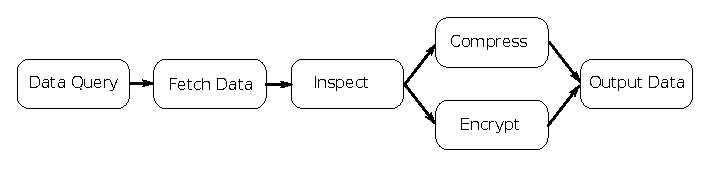
\includegraphics[width=3.5in]{ip-data-proc}
}

\subfigure
{
	\includegraphics[width=3in]{op-data-proc}
}
\caption{Sample stream application}
\label{fig1}
\end{figure}

The main challenge that arises in such a situation is how to tackle such large number of computations from the application and the network operations due to the intensive communication. Two important features enable us to tackle this challenge posed by such a system. Firstly, the operations of both the application and the network is parallel in nature and secondly, the presence of multicore processors to execute the application. 

In our system we use an efficient parallel processing framework that could leverage on multicore processors and multi queue network controllers to achieve this. The performance of multicore processors has dramatically improved the capability of commodity hardware. With this we would be able to meet the computational demand of the application. In addition, the presence of multi queue network interface controller which was designed to handle multiple streams of data could help us achieve the necessary communication performance.

An important part of our system is the tasks related to packets such as Userdatagram Protocol (UDP), Internet Protocol (IP), etc., We utilize the click modular router for these packet processing tasks. Click modular router is a tool that includes a library of elements which is used in building flexible, re-configurable and modular software routers \cite{Kohler2000}. It offers a platform that is flexible for rapid development of newer network protocols and achieves good performance. An improved version known as SMP Click supports thread based parallel processing of network related tasks\cite{Chen:2001:FCP:647055.759948}. Until recently click's performance in the user space was not as good as its kernel space equivalent. This is mainly due to its extensive use of polling driver in the kernel space that was not possible in user space. Netmap I/O\cite{Rizzo:2012:RNI:2090147.2103536} provides a set of APIs that could directly access the packets from the NIC and it helped in the recent improvement of click's user space performance. We found the simpler construction of \texttt{netmap} easier to adapt to our framework compared to other user space packet access APIs \cite{Rizzo:2012:RNI:2090147.2103536} \cite{1564468} \cite{Krasnyansky}.   

Section \ref{dppl} represents the design principles that we follow to conceptualize our framework. Section \ref{imple} describes the implementation details used in the construction of the system. In section \ref{ppe}, we show the challenges involved in using a system consisting of processes that are used to actually perform the work. The extent to which we extract parallelism ranges not only to the packet tasks but to the low level access of data I/O to the network interface hardware through certain additions to the \texttt{netmap} APIs. Finally in Section \ref{app-const} we present a simple application constructed from operations such as compression and encryption in order to evaluate our high-level framework.

\section{Design Principles}
\label{dppl}

The design of a high-level programming framework that integrates packet processing tasks into the application requires overcoming several challenges. \comment{The entire system is driven by the extent to which parallelism can be extracted. Some of the techniques that can be applied to the packet processing tasks can be used for the tasks related to the application.} In this section, we describe these challenges and the principles that are used to tackle them. \comment{We focus on the methodologies related to the packet processing tasks and the parallel processing engine itself.} 

\subsection{Userspace Packet I/O}

For a packet processing system to be integrated with an application it is necessary to have an efficient mechanism for accessing the data from the NIC without interacting with the operating system. Rapid data access here is crucial for the extraction of data parallelism at later stages. \comment{In using the techniques described below we exploit the modern NIC architecture to its full potential.}

\subsubsection{Handling Multiple Hardware Queues}

The development of virtualization and improved network flow handling has lead to hardware level multi queue support in the NICs. During transmission concurrent writes to different queues are possible, enabling multiple processes to send data simultaneously. During reception the NIC classifies the packet on to one of the receive queues using a technique known as Receive Side Scaling (RSS)\cite{micro2008} \cite{intel2010}. It uses the header information or tuples to classify packets on to different hardware queues. Multi queue support can handle several streams of data in parallel and it is exploited extensively in our framework to process data concurrently. By offloading the classification of packets to the NIC, it removes any overhead associated with packet classification in the application. We use these hardware queues as a means of not only accessing the data in parallel but balancing the workload across different threads. This is done by controlling the number of queues that each process handles based on the rate at which packets are received in each of the queues. It is necessary to have different processes accessing the transmit and receive queues to maximize concurrent access to data. 

\subsubsection{Flow based Packet Batching}

Packet batching is a common method used to boost the performance of network applications. Packet batching combines several packets and performing operations on them together, thus reducing the overhead involved in the I/O operations. 

In our framework we utilize batching but the number of packets that forms a batch is not fixed but varies based on the available space in the hardware queue. This number reflects the amount of data we are able to process before issuing hardware synchronization calls and forms a important means by which we reduce the usage of system calls.

\subsubsection{Reduction of Per Packet System Calls} 

System calls are required in order to synchronize data between the NIC hardware and the buffer memory used for intermediate storage of packets. Previous work describe the overhead associated with per packet system calls and provide means of optimizing this\cite{1564468}\cite{Han:2010:PGS:1851275.1851207}\cite{Rizzo:2012:RNI:2090147.2103536}. 

We employ an \textit{adaptive scheme} described in section \ref{ppio} that uses the above principle. Our framework balances the system calls based on the communication rate and application processing speed. The transmission and reception are handled differently to optimize the usage of system calls in each of the case independently. During transmission we issue system calls to synchronize the available buffer space based on the rate at which we transmit data. This prevents degradation in latency for larger packets and improves performance for smaller packets given the same bandwidth at which we transmit in both the cases. During reception of packets the system reads packets at the rate at which it is able to process them.

\subsection{Packet Processing Graph}

\comment{Understanding the set of packet processing tasks associated with the application is essential to performing them in parallel.} We use a graph based representation of packet processing tasks to determine the dependency involved for the different stages and determine the relation with that of the different tasks of the application. The graph contains the stages through which the data, associated with the application, is transformed into network packets and vice versa. It shows which of the tasks can be performed in parallel with those of the application and highlights those that have data dependency on a specific task in the application. This graph also enables optimizations based on the characteristics of the application or the architecture used for execution. Figure \ref{fig2} shows a User Datagram protocol (UDP) packet generation represented in this graph.\\

\begin{figure}[ht]
\centering
\includegraphics[width=3.5in]{pack-op}
\caption{Simplified udp packet construction}
\label{fig2}
\end{figure}

\subsection{Application Task Graph}

\comment{Application task graph represents the operations associated in performing the computations.} The subset of the application that we are interested in parallelizing is the stream processing component. In such components the communication between tasks is predictable and there is correlation between the stages of the application. Both the packet processing and application tasks can be represent by a directed acyclic graph (DAG) similar to the packet processing graph. The packet processing tasks operate on packets and the application tasks operate on the data. Since we focus more on parallel packet processing, the optimization in relation to the application graph are not discussed. It is assumed that a static version of the application graph is available and we focus more on executing these tasks in parallel with that of the packet processing tasks. 

\subsection{Integration}

The sequence of tasks that can be executed in parallel is determined at this stage. The integration stage is used to combine the application graph and the packet processing graph into a larger graph that unifies and represents the overall operations. The dependency relations determined on the previous cases are used in establishing links between the graphs. We determine the sequence of tasks that can be executed in parallel from both the application task graph and packet processing graph. The combined set of tasks is then used by the parallel processing engine. 

\subsection{Parallel Processing Engine}

Two important aspects that the parallel processing engine must tackle is the scheduling of tasks and balancing the load across the available resources. The parallel processing engine consists of processes which are bound to specific core and act as engines to execute the workload. It is constructed in a manner in which its flexible and can adapt to utilize the resources efficiently. The tasks are scheduled across these execution engines based on the available resources and its requirements. In this manner the workload is distributed uniformly while retaining control over the different execution elements. 

\section{Implementation}
\label{imple}

Most of the existing stream applications depend on the operating system for most of their communication tasks. In commodity systems, the interaction with the operating system for network operations is a necessary abstraction to handle multiple applications. However, in the case of specialized servers which cater to specific applications it would be beneficial to interact directly with the network device. Moreover, in the case of intensive network traffic the operating system could act as a bottleneck due to the overhead associated with data flowing through the kernel before being transmitted through the network device\cite{Wu:2007:PPB:1323954.1323957}\cite{Wu:2007:PAL:1227865.1228021}. Eliminating this would be possible by either executing the application in the kernel space which could compromise stability of the system or by using an interface for accessing the NIC buffers from the user space itself. The later case of accessing the buffers of network hardware in user space is supported by several interfaces such as \texttt{netmap} \cite{Rizzo:2012:RNI:2090147.2103536}, PF\_RING DNA \cite{1564468}, UIO-IXGBE \cite{Krasnyansky}, etc., Even though the exported APIs support user space packet access they lack the ability to be invoked in a efficient manner by the application. The lack of support for interacting with these APIs in order to read and write data in parallel from the different process or threads adds to this problem. Moreover since the application is responsible for handling network packets it has to perform the additional operations that would otherwise be carried out by the operating system. 

The framework provides support for sending and receiving data in parallel over the network interface from user space and a common parallel execution engine that supports both the application and packet processing tasks. 

\subsection{Parallel Packet I/O}
\label{ppio}
The parallel packet I/O interface when combined with the application tasks provides concurrent communication by the application threads or processes over the network. To do this two important requirements are to be met. Firstly, it should provice access to network data from user space which we can write to in parallel and secondly, to integrate it with the application by providing necessary interfaces for performing the packet operations.

\subsubsection{Userspace Packet Access}
Applications executed in the kernel space for accessing hardware devices directly would lead to instability of the entire system. Instead, several previous work \cite{Rizzo:2012:RNI:2090147.2103536}, \cite{1564468}, \cite{Krasnyansky}, etc., propose access of network buffers from user space. We use \texttt{netmap} APIs \cite{Rizzo:2012:RNI:2090147.2103536} to access data from the network buffers. \texttt{Netmap} uses a set of ring buffers in the kernel space and user space to export the network hardware buffer's memory region. This enables the applications to execute in the user space and directly access the network hardware. It prevents the application from accessing memory outside the valid region by checking limits of the ring buffer. Packets can be written to the buffers when the space is available and an \textit{ioctl} call to the driver would enable the network controller to send the data. A \textit{poll} interface is implemented on the memory region mapped in the user space to check when new packets are available. On reading or writing the packets the available space is updated. 

We leverage on the availability of multiple hardware queues present in modern NIC to read and write data concurrently to the hardware. \texttt{Netmap} by default supports assigning each hardware queue to an individual application process or thread, but we noticed that in order to be efficient in handling the interface we had to assign more than one queue to a particular thread or process. We modified \texttt{netmap}'s hardware queue assignment API to support this. Later, it also allowed the framework to balance the amount of packets handled by each process by varying the number of queues assigned to each of it in order to balance the workload.

We also found that it was essential to have a balanced control over issuing the system calls with respect to the amount of data being transferred. Frequent system calls seem to hamper the bandwidth and latency and in essence affect the peak performance of the application. To tackle this we propose the following algorithms for reading and writing data from the hardware queues using the \texttt{Netmap} APIs. The algorithms are designed to provide these features,

\begin{itemize}

\item Provide batching of packets based on available space on hardware rings
\item Reduce the usage of system calls such as \textit{ioctl \& poll}
\item Mechanisms for handling multiple queues through the application

\end{itemize}

By minimizing the synchronizations with the hardware rings we essentially limit the system calls issued and improve the overall system performance. 

\begin{algorithm}
\caption{To send packets}
\label{s_pack}
\begin{algorithmic}[1]

\State \textbf{struct} $ring[ n ]$\textbf{\{}
\State \Comment{Stores information about hardware rings}
\State \Comment{ $ n \gets \ $tx\ rings\ assigned\ to\ thread}
\State \  \  $avb$, available space
\State \  \  $curr$, current position
\State \  \  $limit$, total space \ \textbf{\}}

\Function{send\_data\_mqueue}{Ring $f(n)$, Data $packet$}
\While{$!success$}
	\State $i \gets f( n ) $ \label{s_pack_param}
	\State $success = $ \texttt{SEND\_DATA}($ i, packet $)
\EndWhile
\EndFunction
\Function{send\_data}{Ring $i$, Data $packet$}
\If{ $ring[ i ].avb > 0$ }
	\State $hw\_ring[ i ].slot( ring[ i ].curr ) \gets packet$
	\State $ring[ n ].avb \gets ring[ i ].avb - 1$
	\State $ring[ i ].curr++$
	\If{ $ring[ i ].avb == 0$ }
		\State $hw\_ring[ i ].avb \ -=\ ring[ i ].limit$
		\State $hw\_ring[ i ].curr \gets ring[ i ].curr$
	\EndIf
	\State \textbf{return} $success$
\EndIf

\State \textbf{\textit{issue ioctl and poll}}
\State $ring[ i ].avb \gets hw\_ring[ i ].avb$
\State $ring[ i ].limit \gets hw\_ring[ i ].avb$
\EndFunction

\end{algorithmic}
\end{algorithm}


Algorithm \ref{s_pack} \& \ref{r_pack} uses a batch update for sending and receiving packets based on the rate at which data flows through the interface. This is done by maintaining a data structure that has the information about the hardware rings and updating it on a periodic basis. Once a fixed amount of space is determined we update this on our local structure, we then continue to read or write data from the hardware ring but update the actual limits and position on our local structure. When we have used up the space that was allocated we then update the hardware ring with the changes done. In cases where the application is generating sparse traffic it would be possible to frequently update the ring in order to maintain a consistent latency in transmission. Multi queue support is provided by managing the process of selecting the ring to send or receive packets based on a application determined function. The $f(n)$ present in Algorithm \ref{s_pack} line \ref{s_pack_param} and Algorithm \ref{r_pack} line \ref{r_pack_param} represents this. Choosing a random queue usually proves to be effective in our experiments but if the application requires a specific flow to be maintained a different function here could provide that support. Cases where this would be helpful is if the data operations are more predictable or if the transactions seem to follow a specific pattern. The $threshold$ specified in Algorithm \ref{r_pack} line \ref{r_pack_thres} is determined for each application based on the rate at which it is able to process data. By issuing the system calls such as \textit{ioctl} and \textit{poll} only when required and effectively handling the multiple queues we are able to achieve improved performance.

\begin{algorithm}[h]
\caption{To receive packets}
\label{r_pack}
\begin{algorithmic}[1]

\State \textbf{struct} $ring[ n ]$\textbf{\{}
\State \Comment{Stores information about hardware rings}
\State \Comment{ $ n \gets \ $rx\ rings\ assigned\ to\ thread}
\State \  \  $avb$, available packets
\State \  \  $curr$, current position
\State \  \  $limit$, total packets \ \textbf{\}}

\Function{receive\_data\_mqueue}{Ring $f(n)$} 
\While{$!packet$}
	\State $i \gets f( n ) $ \label{r_pack_param}
	\State $packet =$ \texttt{RECEIVE\_DATA}(Ring $i$)
\EndWhile
\EndFunction

\Function{receive\_data}{Ring $i$}
\If{ $ring[ i ].avb > 0$ }
	\State $packet \gets hw\_ring[ i ].slot( ring[ i ].curr ) $
	\State $ring[ i ].avb \gets ring[ i ].avb - 1$
	\State $ring[ i ].curr++$
	\If{ $ring[ i ].avb < threshold$ } \label{r_pack_thres}
		\State $hw\_ring[ i ].avb -= ring[ i ].( limit - avb)$
		\State $hw\_ring[ i ].curr \gets ring[ i ].curr$
		\State $ring[ i ].avb \gets hw\_ring[ i ].avb$
		\State $ring[ i ].limit \gets hw\_ring[ i ].avb$
	\EndIf
	\State \textbf{return} $packet$
\EndIf

\State \textbf{\textit{issue ioctl and poll}}
\State $ring[ i ].avb \gets hw\_ring[ i ].avb$
\State $ring[ i ].limit \gets hw\_ring[ i ].avb$
\EndFunction

\end{algorithmic}
\end{algorithm}



\subsubsection{Packet Processing Operations}

Packet processing operations consists of converting the raw data that the application provides into network packets suitable for transmission. Since the application tasks are represented as a set of operations on a stream of data we include these operations as stages through which the data flows through to get transformed into data packets. By integrating them with the application task graph it makes it easier to extract parallelism later in the execution engine. Several user space libraries exist that perform packet related processing operations like libnids \cite{libnids}, lwip \cite{Dunkels01designand}, click \cite{Kohler2000} etc., Since our application are targeted at a closed environment, we chose the click modular router for its flexibility and vast library of elements as a means of operating on the network packets. Our current framework supports a simpler udp protocol but click's modular infrastructure would make it easier to construct more complex ones.

Each of the element in the click contains a virtual function which is called from the previous element it is attached to. We had to overcome this limitation of using click's infrastructure to construct based on dynamically initialized objects and virtual functions. This was necessary due to two important conditions, one was to eliminate the overhead associated with the dynamic construction of the objects and virtual functions and the other was to optimize the task graph along with these operations. To achieve this our framework constructs a simpler support structure that can link elements supported in click and import them to integrate with our application.

\subsection{Parallel Processing Engine}

After integrating the packet operations by means of support from \texttt{click}'s infrastructure and data access to network hardware through \texttt{netmap}'s APIs, we integrate these operations with the application graph, we now have a complete task graph that does both the computation and communication operations. The next logical step was executing these tasks in parallel. Two basic forms in which we can extract this lies in data and task parallelism. Packet streams have an inherent nature to operate in a data parallel fashion i.e. it is possible to operate on two different streams simultaneously. Since the application tasks in turn depend on the data packets they could also be executed in parallel. So from the integrated graph constructed by combining the application and packet processing operations it becomes possible to extract data parallelism by operating on different data streams simultaneously. In executing different graphs that represent distinct operations on the data streams it is possible to exploit task parallelism.

\subsubsection{Execution engine}
\label{ppe}

The execution engine consists of set of process and threads that the work is scheduled upon in order to be executed. When implementing threads to execute code which consists of system calls to the OS such as \textit{malloc(), ioctl(), poll(),} etc., we found a degradation in performance even when the work that has to be executed is completely independent. To support the light weight style of threads the OS implements most of the locking mechanisms for system calls coming from threads. Previous research such as \cite{Lever:2000:MPM:1267724.1267780} \cite{Dice:2002:MLM:773039.512451} \cite{Michael:2004:SLD:996893.996848} shows the degradation in performance due to the usage of \textit{malloc()} in threads. Since our framework has to deal with system calls and issue them in parallel we use \textit{unix process} to perform the tasks concurrently. We do this by using \texttt{Message Passing Interface (MPI)} \cite{TheMPIForum:1993:MMP:169627.169855} to construct a set of processes that is scheduled on to the different cpus on a multicore system.

In order to prevent interference from the OS scheduler's process migration, we specify \textit{affinity} of the MPI process on to particular cpu cores. This prevents our process from being executed on a different cpu other than that specified. This makes our processes act as execution engines running on each of the cores on which we schedule the operations that are to be performed. Several previous research\cite{Salehi:1996:EAS:234766.234769}\cite{1409136} show the importance of affinity in network sensitive applications. Next, from utilizing our \textit{Parallel Packet I/O} we specify the hardware queues each of these process handle. Initially we divide the queues evenly among the different processes we create, but later during execution we could modify the allocation based on the application operations scheduled on them. Our modifications to \texttt{netmap}'s hardware queue assignment API help us here in redistributing the queues to different processes. In using \texttt{MPI's send \& receive} inter-process communication calls it makes it possible to modify the attributes of the process such as the cpus assigned or the number of queues it handles and even modify the operations the processes were initially assigned.

\subsubsection{Parallel task processing}
\label{ppt}

Once we have scheduled our execution engines on the physical system, the next step is to execute the integrated task graph consisting of application and packet operations on them. To extract data parallelism we replicate the task graph on to the multiple execution engines. This is to ensure operations on the same data are performed on the same cpu thereby reusing local cache. By making sure that packets belonging to specific flow always end up in the same execution engine, we only perform operations conforming to that stream of data. We leverage on the ability of modern network to classify packets, based on attributes of the packet, on to different queues.


\lstset{language=C,caption={Packet Payload Modification Function},label=payload_sub}
\begin{lstlisting}
bool payload_copy( const void *payload_data, uint32_t length )
{
    uint32_t headroom = _data - _head;
    uint32_t tailroom = _end - _tail;
    uint32_t orig_length = _tail - _data;
    uint32_t n = length + headroom + tailroom;
    if( n < min_buffer_length ) 
    {
        tailroom = min_buffer_length - length - headroom;
        n = min_buffer_length;
    }
    _data = _head + headroom;
    _tail = _data + length;
    if( payload_data )
        memcpy( _data, payload_data, length );
    return true;
}
\end{lstlisting}


In order to replicate the task graph we had to overcome some restrictions. First was to ensure that there was no intricate data dependency between different data streams. Although, click's library of elements are designed to be executed in parallel \cite{Chen:2001:FCP:647055.759948}, it was more oriented towards being executed in a serial fashion. Hence we had to ensure the code present in the elements were thread safe. One important modification we had to perform was in the packet library that click uses. Click by default destroys and re creates the packet's internal storage buffer by reallocating memory space, which is an expensive operation. In order to avoid this overhead we allocate a packet with a large static buffer and copy the data to be modified on it. We modify the pointers that determine the header and data addresses based on the required packet length. This is done by using a simple sub routine shown in Listing \ref{payload_sub} that we added to the click's packet library. Even though this incurs the overhead of a copy operation it does avoid performing invalid and dangerous memory operations directly on the network hardware queue's buffer.

Click's packet library does provide a mechanism to take ownership of a specific address and pass a destructor to be called when the packet is killed. To prevent corruption of memory mapped from the hardware queue by the application tasks we use the above mechanism to copy the data before modifying it. In generating the application graph as a sequence of operations it also makes it possible to run different graphs on each individual execution engine. The MPI inter-process communication is used to schedule the application and packet operations on the processes representing the execution engines. Further more, we use it to also perform explicit data sharing on tasks in the application that requires it.

\section{Experimental Evaluation}

The evaluation of our system should test the scalability and the performance speedup that we could achieve on a multicore system for an application that is constructed in our framework. To do this we choose two generic operations such as compression and encryption, built simple stream applications based on them in our framework. We then measured the improvement in performance as we increased the number of execution engines that are dedicated for the application.

\subsection{Hardware Setup}

The multicore system that is used to evaluate the framework consists of two servers connected directly to each other. Each of the server consists of two Intel Xeon 5600 hexacore HT in a dual socket configuration with 24GB DDR3 memory. So there is a total of 2 Processors x 6 Cores x 2 HT = 24 cpus in each server. These servers are connected with each other using Intel 8299EB 10Gbe adapters over direct attach twinaxial cables. They are placed in PCI Express x8 slot in each system to maximize the available bandwidth for the cards. This forms a closed connection between two servers and limits the influence of any external devices such as switches or routers on the actual data transmission. 

The application is constructed as two parts, one acting as a source of data and other a sink. We measure the overall time it takes for application task operations, packet operations and the time to send from the source and receive at the sink. This is done for different packet sizes and applications. Then we plot the speedup achieved in each of the cases over the serial version where we have a single sender and receiver operating on the multiple queues. This is considered to be the baseline in our experiments since this is similar to how the OS behaves for transmitting and receiving using the multi queue network controller.

The Intel 82599EB has limitations on the number of queues it can use for Receive Side Scaling (RSS) which is restricted to 16. So this limited our maximum amount of processes at the sink to be 16 even though there were 24 cpus available on the system. The source is not affected by this limitation and can scale to all the 24 cpus available on the system with the presence 24 hardware tx queues. Overall we at least have one hardware queue mapped to each of our processes or execution engines. We also ensure that each of the processes are bound to a particular cpu by issuing affinity call to the OS to ensure that we are not migrated between different cores.

\subsection{Application Construction}
\label{app-const}

In order to evaluate our framework we needed distinct operations that would be suitable to be applied in a streaming framework. Since compression and encryption applications are used commonly we chose two applications that represent these operations. The integrated graph that represents both these applications are shown in fig \ref{fig-app-graph}. Since our intention is to test the overall performance of the stream applications we use simple protocol such as udp in order to send data between the source and the sink.

\begin{figure}[htb]
\centering
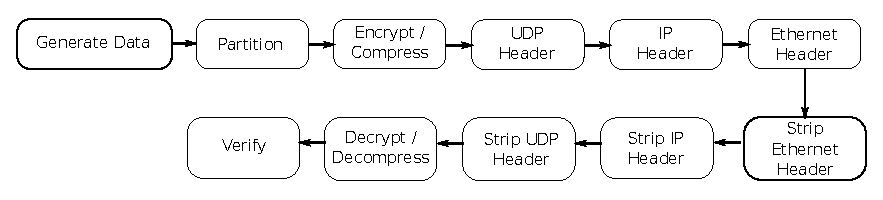
\includegraphics[width=3.5in]{enc-dec}
\caption{ Integrated Task Graph  }
\label{fig-app-graph}
\end{figure}

Both the applications are constructed in a similar way. Two data sizes of 1.28 GB and 2.56 GB are selected as the workload for the compression and encryption applications respectively. Openssl library is used for the encryption and decryption and zlib is used for the compression and decompression operations respectively. The application consists of data generation phase after which it is compressed or encrypted depending on the application after which the packet operations are done. At this point the stream consisting of packets is sent over the network using the multiple queues. The sink side does the reverse of these operations. Once the data is received the packet operations are performed to extract the payload, after which the decompression or decryption operation is performed to retrieve the original data. These are some of the basic operations that would be required to construct a much more complex application. In choosing to compare these simple operations we avoid any limitations that might be present in a more complex application. This would enable us to evaluate the performance due to our framework and not that of any optimization done in the application.\\

\begin{figure*}[tb]
\centering
\includegraphics[width=7in]{result}
\caption{Performance Speedup; (a),(b),(c) - Application A. Encryption; (d),(e),(f) - Application B. Compression;\\ \newline Speedup based on time in takes to compute a fixed workload for different number of source and sink processes\\ \newline and for varying packet sizes over a single source and sink are shown above}
\label{fig-res}
\end{figure*}

\section{Results}

We see that there is considerable difference in the way each of the operations behave as we scale them. This is shown in Figure \ref{fig-res}. We can make three distinct observations from the results. \\

One is that from fig\ref{fig-res}.(d,e,f) we find that the compression requires a lot more work than that of decompression, whereas from fig\ref{fig-res}.(a,b,c) encryption and decryption seems to be more or less balanced. This is evident from the continued speedup we get up to 4 senders in the case of compression \& decompression. In encryption \& decryption this trend is not seen and the performance only improves by increasing both the number of senders and receivers. So we conclude that the combination of parallel tasks for application and packet operations differs between different applications. Determining this for each scenario is essential to boost the performance of the overall system.\\

We see that the packet sizes have some impact on the performance from fig\ref{fig-res}.(d,e,f) but there is not much change compared to the overall speedup we achieve in each of the case. It can also be noticed that the compression operation seems to be influenced more than that of encryption operation. There seems to be speedup of 12x from fig\ref{fig-res}.(d) in the case of smaller packets and 10x from fig\ref{fig-res}.(f) for larger packets for compression operation. Whereas in the encryption application there is not much change and we get a speedup of 8x for any packet size observed from fig\ref{fig-res}.(a,b,c). While, packet sizes seem to have a much larger effect when there are smaller number of senders or receivers, but for larger cases not much change is observed in fig\ref{fig-res}.(d,e,f). So we conclude that the influence of a parameter for the network system such as a packet size varies between different applications and it is essential to have a unified system that can tackle both the operations together.

From fig\ref{fig-res}(a,b,c,d,e,f), we noticed the drop in speedup as we move from 12 senders to more. This could be due to the influence of NUMA architecture \cite{Awasthi:2010:HPO:1854273.1854314} on the performance of the system. This is the particular point in which we utilize all the cores of a particular cpu and move on to a different socket. Mainly, the combination of cache locality and limitation of the network controller to receive data through the PCI-E bus from both the processors could be the contributing factors. Still, we find that even in a NUMA architecture once our framework overcomes the initial drop, it continues to improve and eventually attain better performance in most cases.

We can see that our framework scales very well for the different workloads provided and can handle both the computations and communication and operate on them in parallel. In some cases we find that our framework could be improved by having a much more control over the fine grained parallelism within the execution engines. This could be done by introducing pipeline stages for the different operations.

\section{Related Work}

Several prior research \cite{Dobrescu09routebricks:exploiting}\cite{Han:2010:PGS:1851275.1851207}\cite{Wang:2009:PPN:1542275.1542307}\cite{springerlink:10.1007/s11227-011-0579-3} have worked on using commodity multicore processors to perform network operations. 

Dobrescu et al.\cite{Dobrescu09routebricks:exploiting} shows the performance improvement achieved in the construction of software routers by distributing the related operations over multiple servers. 

Han et al. \cite{Han:2010:PGS:1851275.1851207} perform tasks related to high performance packet processing on commodity hardware using GPUs. They have developed a novel framework know as PacketShader that can do packet processing in user space by exploiting massively-parallel architecture of GPUs. 

Wang et al. \cite{Wang:2009:PPN:1542275.1542307} constructs a high performance connection-affinity based lock-free multicore network processing system that claims to achieve multiple Gbps network processing speed for complex tasks. 

Egi et al.\cite{springerlink:10.1007/s11227-011-0579-3} shows techniques on parallelizing network operations on multicore architectures by defining principles that consider multiple resources and not just the CPU alone.

Stream programming languages such as StreamIt \cite{Thies:2002:SLS:647478.727935}, LUSTRE \cite{Halbwachs91thesynchronous}, etc., target stream applications but they focus more on parallelizing the computations related to the application alone on the multicore system.

\comment{
All of these applications are more focused on operating as a network application and primarily focus on parallelizing packet operations. In our work even though a part of it involves parallelizing network operations, the objective of this research is to provide support for parallelizing stream application and distributing their workloads over multiple systems. This also requires optimizing the underlying network operations by parallelizing it.}

\texttt{Netmap} \cite{Rizzo:2012:RNI:2090147.2103536}, provides the APIs to access the hardware queue's buffer in user space by means of memory mapped rings. It implements an intermediate ring in kernel space that is used to synchronize the data from the user space to that of hardware queues in the NIC. 

Click modular router \cite{Kohler2000} is an extensively used tool for the construction of software routers using general purpose hardware and provides a massive infrastructure to support this. SMP Click \cite{Chen:2001:FCP:647055.759948} is an improved version, which supports parallel processing of these using threads. Click implements its own mechanism and polling driver in kernel space to access packets, bypassing the operating system's network infrastructure.


\comment{
In order to send data the programmer calls \textit{poll} on the tx ring in user space and writes to it when space is available. Then he calls \textit{ioctl} to synchronize the data with the kernel ring and transmit the data. To receive the packets \textit{poll} is again called on the rx ring in user space but this time to check for new data and after reading it, he issues \textit{ioctl} to let the driver know that packet has been read and space can be re used.


, our framework uses techniques as described in Section \ref{imple} to integrate them with the application and access them in parallel from different application processes. Also, while some of click's \cite{Kohler2000} elements are used to provide support for packet processing operations, in our framework we use it for doing some of application's network tasks alone. Due to this we modified a subset of click's elements in order to support our system.


 In our framework we target a different category of stream applications such as data mining, real time image analysis, etc., which tend to compute on large amounts of data. In order to improve overall performance in such cases, the operations are distributed over multiple systems. Our framework provides an easier methodology to construct such an application while managing both the parallelizing and communication operations.

Our framework provides the necessary functionality to target communication intensive stream applications. We focus on improving the overall performance of such an application by integrating the network and application operations. We do this by providing a high-level programming framework that can be used to construct these applications, which can extract parallelism and improve communication performance. Using this it would be possible to develop stream applications that could be distributed over multiple systems and using our framework it would be possible to handle the highly intensive communication between them.}

\section{Conclusions}
In this paper we have proposed a high-level programming framework that can integrate packet processing within stream applications and perform both the operations in parallel. 

We conclude that by using our algorithms for sending and receiving data, which implicitly performs batching and reduces the usage of system calls, and in combining this with \texttt{netmap} APIs which minimizes the interaction with the operating system, communication performance in our framework never becomes the bottleneck in our system on the programs we have tested. Instead of performing the packet operations in the OS, by integrating it with the application using click's elements within our infrastructure we are able to construct a unified task graph that represents the computation and communication operations. Using this we are able to parallelize these operations together and achieve speedups of more than a factor of eight in all the applications we tested. 

In integrating these features into a programming framework, the system of multiple queues, parallel communication and computation are entirely hidden from the programmer, who merely specifies a standard stream graph for computation alone. The results shows that our system scales well to as many as 24 parallel processes on a multicore computer, and achieves speedups of more than a factor of ten in some cases compared to sequential versions of the stream applications.

% An example of a floating figure using the graphicx package.
% Note that \label must occur AFTER (or within) \caption.
% For figures, \caption should occur after the \includegraphics.
% Note that IEEEtran v1.7 and later has special internal code that
% is designed to preserve the operation of \label within \caption
% even when the captionsoff option is in effect. However, because
% of issues like this, it may be the safest practice to put all your
% \label just after \caption rather than within \caption{}.
%
% Reminder: the "draftcls" or "draftclsnofoot", not "draft", class
% option should be used if it is desired that the figures are to be
% displayed while in draft mode.
%
%\begin{figure}[!t]
%\centering
%\includegraphics[width=2.5in]{myfigure}
% where an .eps filename suffix will be assumed under latex, 
% and a .pdf suffix will be assumed for pdflatex; or what has been declared
% via \DeclareGraphicsExtensions.
%\caption{Simulation Results}
%\label{fig_sim}
%\end{figure}

% Note that IEEE typically puts floats only at the top, even when this
% results in a large percentage of a column being occupied by floats.


% An example of a double column floating figure using two subfigures.
% (The subfig.sty package must be loaded for this to work.)
% The subfigure \label commands are set within each subfloat command, the
% \label for the overall figure must come after \caption.
% \hfil must be used as a separator to get equal spacing.
% The subfigure.sty package works much the same way, except \subfigure is
% used instead of \subfloat.
%
%\begin{figure*}[!t]
%\centerline{\subfloat[Case I]\includegraphics[width=2.5in]{subfigcase1}%
%\label{fig_first_case}}
%\hfil
%\subfloat[Case II]{\includegraphics[width=2.5in]{subfigcase2}%
%\label{fig_second_case}}}
%\caption{Simulation results}
%\label{fig_sim}
%\end{figure*}
%
% Note that often IEEE papers with subfigures do not employ subfigure
% captions (using the optional argument to \subfloat), but instead will
% reference/describe all of them (a), (b), etc., within the main caption.


% An example of a floating table. Note that, for IEEE style tables, the 
% \caption command should come BEFORE the table. Table text will default to
% \footnotesize as IEEE normally uses this smaller font for tables.
% The \label must come after \caption as always.
%
%\begin{table}[!t]
%% increase table row spacing, adjust to taste
%\renewcommand{\arraystretch}{1.3}
% if using array.sty, it might be a good idea to tweak the value of
% \extrarowheight as needed to properly center the text within the cells
%\caption{An Example of a Table}
%\label{table_example}
%\centering
%% Some packages, such as MDW tools, offer better commands for making tables
%% than the plain LaTeX2e tabular which is used here.
%\begin{tabular}{|c||c|}
%\hline
%One & Two\\
%\hline
%Three & Four\\
%\hline
%\end{tabular}
%\end{table}


% Note that IEEE does not put floats in the very first column - or typically
% anywhere on the first page for that matter. Also, in-text middle ("here")
% positioning is not used. Most IEEE journals/conferences use top floats
% exclusively. Note that, LaTeX2e, unlike IEEE journals/conferences, places
% footnotes above bottom floats. This can be corrected via the \fnbelowfloat
% command of the stfloats package.

% conference papers do not normally have an appendix


% use section* for acknowledgement
\section*{Acknowledgment}
This work is funded by the IRCSET Enterprise Partnership Scheme in collaboration with IBM Research, Ireland.

% trigger a \newpage just before the given reference
% number - used to balance the columns on the last page
% adjust value as needed - may need to be readjusted if
% the document is modified later
%\IEEEtriggeratref{8}
% The "triggered" command can be changed if desired:
%\IEEEtriggercmd{\enlargethispage{-5in}}

% references section

% can use a bibliography generated by BibTeX as a .bbl file
% BibTeX documentation can be easily obtained at:
% http://www.ctan.org/tex-archive/biblio/bibtex/contrib/doc/
% The IEEEtran BibTeX style support page is at:
% http://www.michaelshell.org/tex/ieeetran/bibtex/
\bibliographystyle{IEEEtran}
% argument is your BibTeX string definitions and bibliography database(s)
\bibliography{IEEEabrv,ref.bib}
%
% <OR> manually copy in the resultant .bbl file
% set second argument of \begin to the number of references
% (used to reserve space for the reference number labels box)
%\begin{thebibliography}{1}

%\end{thebibliography}

% that's all folks
\end{document}





